\documentclass[12pt]{article}
\usepackage{geometry}                % See geometry.pdf to learn the layout options. There are lots.
\geometry{letterpaper}                   % ... or a4paper or a5paper or ... 
%\geometry{landscape}                % Activate for for rotated page geometry
\usepackage[parfill]{parskip}    % Activate to begin paragraphs with an empty line rather than an indent
\usepackage{daves,fancyhdr,natbib,graphicx,dcolumn,amsmath,lastpage,url}
\usepackage{amsmath,amssymb,epstopdf,longtable}
\usepackage{paralist}  % need to properly formulate standard answer blocks
\usepackage[final]{pdfpages}
\DeclareGraphicsRule{.tif}{png}{.png}{`convert #1 `dirname #1`/`basename #1 .tif`.png}
\pagestyle{fancy}
\lhead{CE 3305 Fluid Mechanics; Exercise Set 3}
\rhead{Name:\_\_\_\_\_\_\_\_\_\_\_\_\_\_\_\_\_\_\_\_\_\_\_\_\_\_\_\_\_\_\_\_\_\_}
\lfoot{REVISION A}
\cfoot{}
\rfoot{Page \thepage\ of \pageref{LastPage}}
\renewcommand\headrulewidth{0pt}
%%%%%%%%%%%%%%%%%%%%%%%%%%%%%%%%%%%%
\begin{document}
%%%%%%%%%%%%%%%%%%%%%%%%%%%%%%%%%%%
\begingroup
\begin{center}
{\textbf{{ CE 3305 Engineering Fluid Mechanics} \\ Exercise Set 3 \\ Summer 2015 -- GERMANY} }
\end{center}
\endgroup
\begingroup
~\newline

\begin{enumerate}
\item (Problem 2.37 pg 57)
Figure \ref{fig:FallingCylinderViscosity} is a schematic of a cylinder falling inside a pipe that is filled with oil.
The annular space between the cylinder and the pipe is lubricated with an oil film that has viscosity $\mu$.
\begin{enumerate}[a)]
\item Derive a formula for the steady rate of descent of a cylinder with weight $W$, diameter $d$, and length $l$ sliding inside a vertical smooth pipe that has inside diameter $D$.
Assume the cylinder remain concentric with the pipe as it falls.
\item Use the general formula you develop to estimate the rate of descent for a cylinder 100 millimeters in diameter that slides inside a 100.5 millimeter inside diameter pipe. 
The cylinder is 200 millimeters long and weighs 15 Newtons.  The lubricant is SAE 20W oil at 10$^o$C.
\end{enumerate}
\begin{figure}[htbp] %  figure placement: here, top, bottom, or page
   \centering
   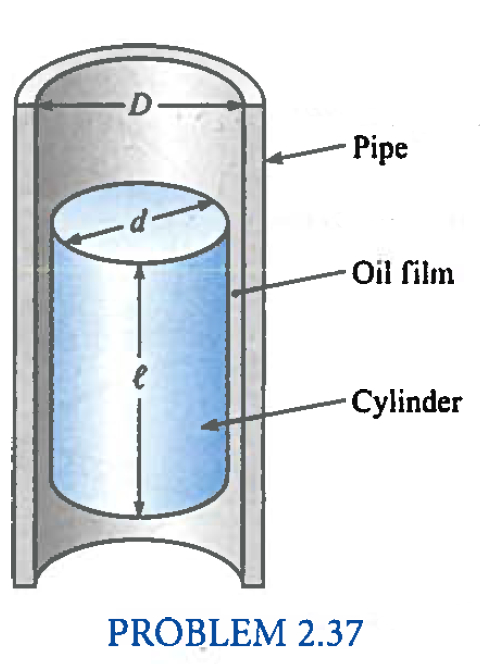
\includegraphics[width=1in]{FallingCylinderViscosity.jpg} 
   \caption{Falling cylinder in an oil-filled pipe}
   \label{fig:FallingCylinderViscosity}
\end{figure}
\clearpage
~
\clearpage
\item (Problem 2.61 pg 59)
Figure \ref{fig:ParallelPlates} is a schematic of two glass plates spaced 1 millimeter apart.  
Calculate the maximum capillary rise of water between the two plates. 
\begin{figure}[htbp] %  figure placement: here, top, bottom, or page
   \centering
   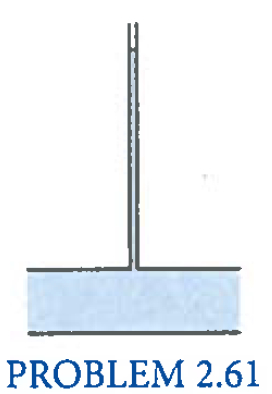
\includegraphics[width=1in]{ParallelPlates.jpg} 
   \caption{Parallel plates immersed in water}
   \label{fig:ParallelPlates}
\end{figure}

\end{enumerate}


\end{document}  